\documentclass[
  dvipdfmx,
]{standalone}
\usepackage{tikz}
\usetikzlibrary{spath3}
\usetikzlibrary{knots}
\usetikzlibrary{hobby}
\usetikzlibrary{patterns}
\begin{document}
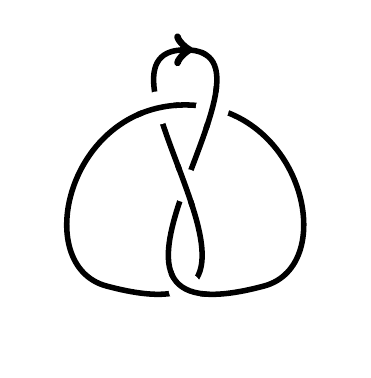
\begin{tikzpicture}
    \begin{knot}[
      consider self intersections=true,
      ignore endpoint intersections=false,
      % draft mode=crossings,
      every strand/.append style={line width=2pt},
      flip crossing=3,
      clip radius=6pt,
      clip width=7,
      % background color=red!20,
    ]
    \strand (0,3)
    .. controls +(0:1.5) and +(195:3) .. (1,0)
    .. controls +(15:1) and +(0:1.5) .. (0,2.3)
    .. controls +(180:1.5) and +(165:1) .. (-1,0)
    .. controls +(-15:3) and +(180:1.5) .. (0,3);
    \end{knot}
  \draw[->, line width=3pt] (0,3) -- ++(0.1,0);
  \end{tikzpicture}
\end{document}